\documentclass{ujarticle}
\usepackage{ketpic,ketlayer}
\usepackage{amsmath,amssymb}
\usepackage{graphicx}
\usepackage{xcolor}
\usepackage{bm,enumerate}
\usepackage[dvipdfmx,colorlinks=true,urlcolor=blue]{hyperref}

\setmargin{20}{20}{15}{20}

\西暦

\renewcommand{\labelitemi}{・}
\pagestyle{empty}

\begin{document}

\begin{center}
KeTCindyのインストール
\end{center}

\vspace{-5mm}

\hfill 修正日:\today

\begin{enumerate}[\bf\large 1.]
\item Cinderella, R, Maxima (WindowsではSumatraも)をインストールする.

 \begin{itemize}
 \item \url{https://beta.cinderella.de}  (Cinderella)\\
\hspace*{6mm}注)Windowsの場合,右クリックして「管理者として実行」を選ぶ.
 \item \url{https://cran.r-project.org}   (R)
 \item \url{https://sourceforge.net/projects/maxima/files}  (Maxima)
 \item \url{https://www.sumatrapdfreader.org/download-free-pdf-viewer.html} (Sumatra)\\
\hspace*{6mm}注)Sumatraのインストール先は,オプションでProgram Files(またはx86)を指定する.

 \end{itemize}
\item TeXをインストールしていない場合はインストールする.
 \begin{enumerate}[(1)]
 \item TeXLiveを推奨 (2018以降ではketcindyが組み込まれている)
 \item KeTTeXはTeXLiveの軽量版
    \begin{itemize}
    \item 以下からダウンロードできる.\\
    \hspace*{5mm}Mac (kettex.dmg)\\
    \hspace*{10mm}\url{https://www.dropbox.com/s/dc4inuk06t07g26/kettex.dmg?dl=0}\\
    \hspace*{5mm}Windows (kettex.exe)\\
    \hspace*{10mm}\url{https://www.dropbox.com/s/fthw4btjqqs33tc/kettex.exe?dl=0}\\
    \hspace*{5mm}Linux (kettex.tar.xz)\\
    \hspace*{10mm}\url{https://www.dropbox.com/s/vg8p07832e9hzlk/KeTTeX-linux-20171022.tar.xz?dl=0}
     \item 解凍したkettexの保存先 /Application\ (Mac), C:\textbackslash\ (Windows)\end{itemize}
 \end{enumerate}

\item KeTCindyのインストール
  \begin{enumerate}[(1)]
  \item ketcindyをCTAN(\url{https://ctan.org})からダウンロードする.\\
  \hspace*{10mm}ketcindyで検索 $>$ Package ketcindy $>$ Download(フォルダ名はketcindy)
    \begin{itemize}
    \item Repositoryはgithubサイトにある最新版へのリンク\\
        \hspace*{10mm}Clone or download $>$ Download ZIP(フォルダ名はketcindy-master)        \end{itemize}
  \item 中に入っているketcindysettings.cdyをダブルクリック
    \begin{itemize}
    \item 必要なら,実行プログラムをCinderellaに設定する.
   \item 画面が狭ければ,右方向に広げる.
  \item 最初は図が出ないが,設定が完了すると図が表示される.
   \end{itemize}

\vspace{3mm}

\begin{layer}{140}{0}
\putnotese{27}{20}{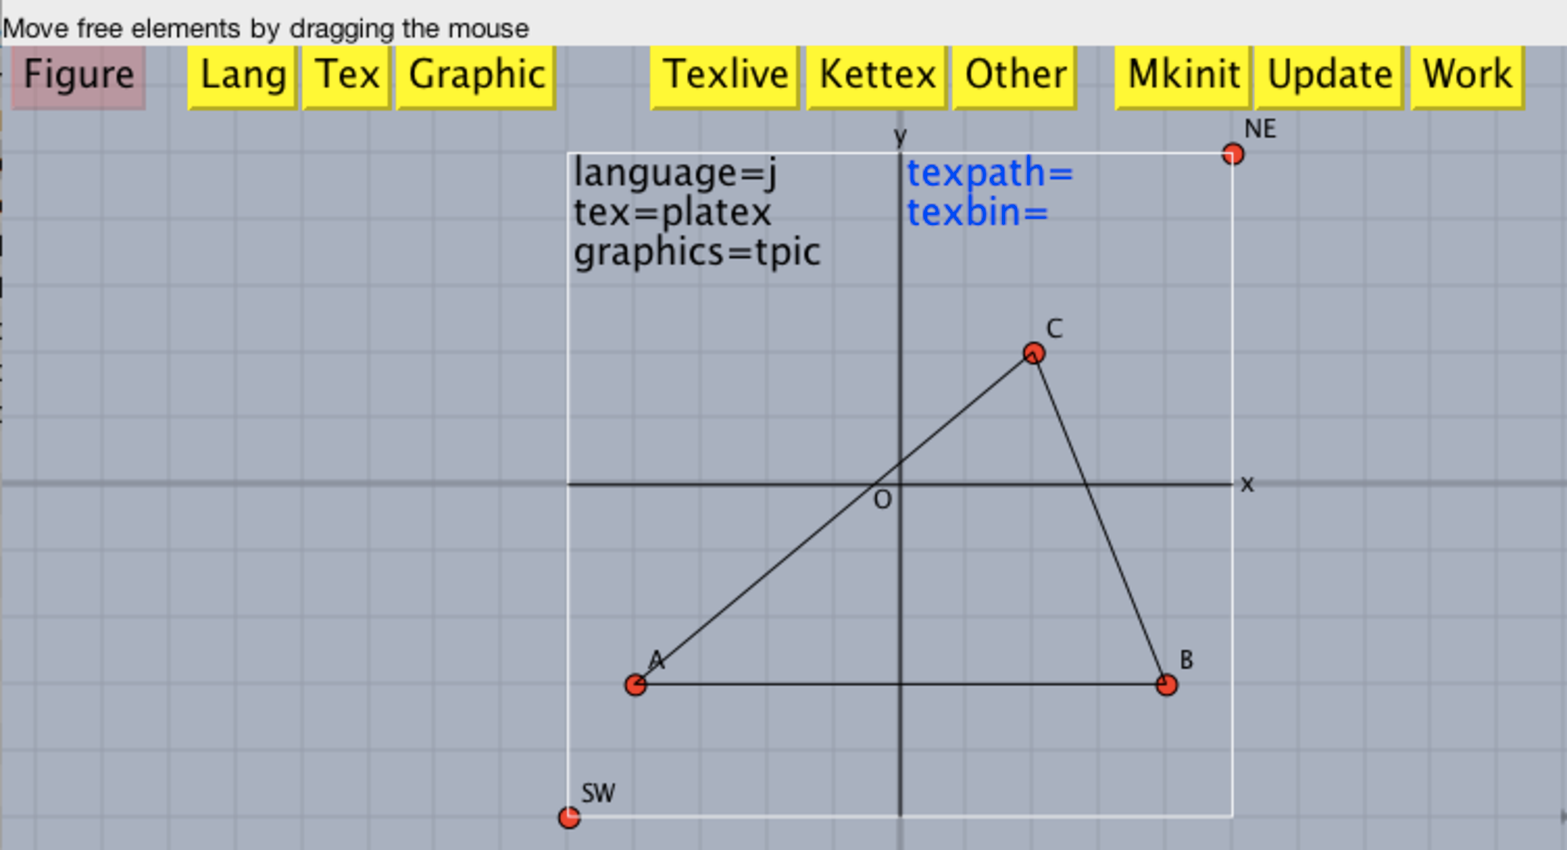
\includegraphics[bb=0.00 0.00 752.00 408.00,width=100mm]{Fig/setting.pdf}}
\putnotee{0}{5}{\bf [1]\ 言語などの選択}
\putnotese{3}{10}{\underline{Language}}
\putnotese{7}{15}{Japanese, English}
\putnotese{3}{20}{\underline{\TeX}}
\putnotese{5}{24}{\begin{tabular}{l}
platex\\uplatex\\latex\\xelatex\\pdflatex\\lualatex\end{tabular}}
\putnotese{3}{58}{\underline{Graphic Code}}
\putnotese{5}{62}{\begin{tabular}{l}tpic\\pict2e\\tikz\end{tabular}}
\arrowline{47}{20}{20}{135}
\putnoten{83}{7}{\bf [2]\ \TeX システムの選択}
\arrowline{83}{20}{13}{90}
\putnotee{125}{5}{\bf [3]\ 作成と更新}
\arrowline{110}{20}{20}{45}
\putnotese{131}{10}{\begin{minipage}[t]{30mm}%
\underline{Mkinit}\\
\hspace*{2mm}ketcindy.iniを\\
\hspace*{2mm}作成する\\
\hspace*{4mm}(User's home)\\
\underline{Update}\\
\hspace*{2mm}ketcindyを更新\\
\underline{Work}\\
\hspace*{2mm}作業フォルダ\\
\hspace*{9mm}ketcindy\\
\hspace*{2mm}を作成する\\
\hspace*{4mm}(User's home)\\
\hspace*{2mm}マニュアルやサン\\
\hspace*{2mm}プルが入っている
\end{minipage}}
\end{layer}

\vspace{77mm}

{\bf [4]\ テストラン}\\
\hspace*{10mm}\verb|Figure|を押す.pdfが表示されれば成功
  \end{enumerate}

\end{enumerate}

\end{document}